\documentclass[12pt, twocolumn, landscape]{beamer}
\usetheme{Warsaw}



%\usepackage[margin=1in]{geometry}  
%\usepackage{graphicx}              
\usepackage{amsmath}               
\usepackage{blindtext}
\usepackage{amsfonts}              
\usepackage{amsthm}                
\usepackage{xcolor}
\usepackage{array}

%\usepackage{titletoc}
\usepackage{pgfplots}
\usepackage{tikz}
\def\checkmark{\tikz\fill[scale=1](0,.35) -- (.25,0) -- (1,.7) -- (.25,.15) -- cycle;} 

%\usetikzlibrary{arrows}v
\usepackage{hyperref}
\hypersetup{
    colorlinks,
    citecolor=blue,
   filecolor=blue,
  linkcolor=blue,
   urlcolor=blue,
   linktoc=all
}




\newtheorem{thm}{Theorem}[section]
\newtheorem{lem}[thm]{Lemma}
\newtheorem{prop}[thm]{Proposition}	
\newtheorem{cor}[thm]{Corollary}
\newtheorem{sol}[thm]{Solution}
\newtheorem{mydef}[thm]{Definition}

\title{\textcolor{lightgray}{3d Rotation with Quaternions}}
\author{\textcolor{lightgray}{Jason Miller}}
\setcounter{secnumdepth}{0} % sections are level 1

\setbeamercolor{normal text}{fg=white,bg=black!90}
\setbeamercolor{structure}{fg=white}
\setbeamercolor{alerted text}{fg=red!85!black}
\setbeamercolor{item projected}{use=item,fg=black,bg=item.fg!35}
\setbeamercolor*{palette primary}{use=structure,fg=structure.fg}
\setbeamercolor*{palette secondary}{use=structure,fg=structure.fg!95!black}
\setbeamercolor*{palette tertiary}{use=structure,fg=structure.fg!90!black}
\setbeamercolor*{palette quaternary}{use=structure,fg=structure.fg!95!black,bg=black!80}
\setbeamercolor*{framesubtitle}{fg=white}
\setbeamercolor*{block title}{parent=structure,bg=black!60}
\setbeamercolor*{block body}{fg=black,bg=black!10}
\setbeamercolor*{block title alerted}{parent=alerted text,bg=black!15}
\setbeamercolor*{block title example}{parent=example text,bg=black!15}

\definecolor{lightred}{rgb}{1.0, 0.01, 0.24}

\begin{document}

%\definecolor{arsenic}{rgb}{0.13, 0.17, 0.19}
%\setbeamercolor{background canvas}{bg = arsenic}
%\color{lightgray}
\date{}
\frame{\maketitle} 

\frame{\frametitle{Why Calculating Rotation in 3d is Valuable: }
\begin{columns}[onlytextwidth]
\column{0.5 \textwidth}
\begin{itemize}
\item Physics Simulations.
\item 3d Animation.
\item Navigation.  
\item And MUCH MORE!
\end{itemize}
\column{0.5 \textwidth}
\visible<2->{
\begin{itemize}
\item Rotation Around Axis.
\item Gimbals.
\end{itemize}
}
\end{columns}
}

\frame{\frametitle{Why They Fail: Rotation Around Axis}
\begin{columns}[onlytextwidth]
\column{0.5 \textwidth}
Left rotation\pause
\column{0.5 \textwidth}
Right rotation
\end{columns}
}

\frame{\frametitle{Why They Fail: Gimbals}
\begin{columns}[onlytextwidth]
\column{0.5 \textwidth}
Normal Gimbal\pause
\column{0.5 \textwidth}
Gimbal Lock
\end{columns}
}

\frame{\frametitle{What We Want}
\begin{center}
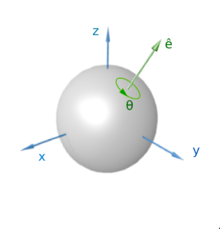
\includegraphics{Ball.png}
\end{center}
}

%CN 1
\frame{\frametitle{Complex Numbers}
$$\textcolor{lightred}{i} * \mathbb{C}$$
\begin{center}
\begin{tikzpicture}[scale=1]
\begin{axis}[
    trig format plots=rad,
    axis equal,
	axis lines = center,
x axis line style = yellow,
y axis line style = red,
x label style={anchor=south},
    y label style={anchor=west},
   xlabel = \( \textcolor{yellow}{(1)} \),
    ylabel = {\( \textcolor{lightred}{i}  \)},
      yticklabels={,,},
      xticklabels={,,}
]
\addplot [color = white] ({1}, {0});
 \addplot[->,line width=1.2pt,color=white,samples=100,domain=0:pi/2] plot({0.9*cos(\x)},{0.9*sin(\x)});
\addplot [domain=0:2*pi, samples=200, white, color = gray] ({cos(x)}, {sin(x)});
\addplot [domain=0:2*pi, samples=200, white, color = white] ({0.05 * cos(x) + 0.9}, {0.05 *sin(x)});
\end{axis}
\end{tikzpicture}
\end{center}
}

%CN 2
\frame{\frametitle{Complex Number Angles}
$$(\cos \theta \textcolor{yellow}{(1)} + \sin \theta \textcolor{lightred}{i}) * \mathbb{C}$$
\begin{center}
\begin{tikzpicture}[scale=1]
\begin{axis}[
    trig format plots=rad,
    axis equal,
	axis lines = center,
x axis line style = yellow,
y axis line style = red,
x label style={anchor=south},
    y label style={anchor=west},
   xlabel = \( \textcolor{yellow}{(1)} \),
    ylabel = {\( \textcolor{lightred}{i}  \)},
      yticklabels={,,},
      xticklabels={,,}
]
\addplot [color = white] ({1}, {0});
 \addplot[->,line width=1.2pt,color=white,samples=100,domain=0:1] plot({0.9*cos(\x)},{0.9*sin(\x)});
\addplot [domain=0:2*pi, samples=200, color = gray] ({cos(x)}, {sin(x)});
\addplot [domain=0:2*pi, samples=200, color = white] ({0.05 * cos(x) + 0.9}, {0.05 *sin(x)});
\addplot [domain=0:0.9, samples = 5, color = white] ({x * cos(1)},{x * sin(1)}) node[below,pos=0.3] {$\theta$};
\end{axis}
\end{tikzpicture}
\end{center}
}


\frame{\frametitle{Introduce Quaternions } 

\begin{columns}[onlytextwidth]

\column{0.5 \textwidth}
\begin{center}Complex Numbers\end{center}
\visible<2->{$$c_0\textcolor{yellow}{(1)} + c_1\textcolor{lightred}{i}$$}
\visible<4->{$$\textcolor{lightred}{i}^2 = -\textcolor{yellow}{1}$$}
\column{0.5 \textwidth}


\begin{center}Quaternions\end{center}
\visible<3->{$$c_0\textcolor{yellow}{(1)} + c_1\textcolor{lightred}{i} + c_2\textcolor{green}{j} + c_3\textcolor{cyan}{k} $$}
\visible<5->{$$\textcolor{lightred}{i}^2 = \textcolor{green}{j}^2= \textcolor{cyan}{k}^2= -\textcolor{yellow}{1}$$}

\end{columns}
\visible<6->{The product of any 2 different complex parts gives the third and they \bf{anti-commute} }
\visible<7->{$$\textcolor{lightred}{i} * \textcolor{green}{j} = -\textcolor{green}{j}*\textcolor{lightred}{i} = \textcolor{cyan}{k}$$}
}

\frame{\frametitle{Times Tables}

\begin{center}
\begin{tabular}{  m{1cm}|| m{1cm}| m{1cm} | m{1cm} | m{1cm} |  } 

* & $\textcolor{yellow}{1}$ & $\textcolor{lightred}{i}$ & $\textcolor{green}{j}$ & $\textcolor{cyan}{k}$  \\ 
  \hline 
\hline
$\textcolor{yellow}{1}$& $\textcolor{yellow}{1}$ & $\textcolor{lightred}{i}$ & $\textcolor{green}{j}$ & $\textcolor{cyan}{k}$  \\ 
  \hline
$\textcolor{lightred}{i}$& $\textcolor{lightred}{i}$ & -$\textcolor{yellow}{1}$ & $\textcolor{cyan}{k}$ & -$\textcolor{green}{j}$  \\ 
  \hline
$\textcolor{green}{j}$& $\textcolor{green}{j}$ & -$\textcolor{cyan}{k}$ & -$\textcolor{yellow}{1}$ & $\textcolor{lightred}{i}$  \\ 
  \hline
$\textcolor{cyan}{k}$& $\textcolor{cyan}{k}$ & $\textcolor{green}{j}$ & -$\textcolor{lightred}{i}$ & -$\textcolor{yellow}{1}$  \\ 
\hline
\end{tabular}
\end{center}

}


\frame{\frametitle{But What About Rotation}
$$\textcolor{lightred}{i} * \mathbb{H}$$
\begin{columns}[onlytextwidth]

\column{0.5 \textwidth}
\begin{center}
\begin{tikzpicture}[scale=0.75]
\begin{axis}[
    trig format plots=rad,
    axis equal,
	axis lines = center,
x axis line style = yellow,
y axis line style = red,
x label style={anchor=south},
    y label style={anchor=west},
   xlabel = \( \textcolor{yellow}{(1)} \),
    ylabel = {\( \textcolor{lightred}{i}  \)},
      yticklabels={,,},
      xticklabels={,,}
]
 \addplot[->,line width=1.2pt,color=white,samples=100,domain=0:pi/2] plot({0.9*cos(\x)},{0.9*sin(\x)});
\addplot [domain=0:2*pi, samples=200, white, color = gray] ({sin(x)}, {cos(x)});
\addplot [domain=0:2*pi, samples=200, white, color = white] ({0.05 * cos(x) + 0.9}, {0.05 *sin(x)});

\end{axis}
\end{tikzpicture}
\end{center}
\column{0.5 \textwidth}
\begin{center}
\begin{tikzpicture}[scale=0.75]
\begin{axis}[
    trig format plots=rad,
    axis equal,
	axis lines = center,
x axis line style = green,
y axis line style = cyan,
x label style={anchor=south},
    y label style={anchor=west},
   xlabel = \( \textcolor{green}{j} \),
    ylabel = {\( \textcolor{cyan}{k}  \)},
      yticklabels={,,},
      xticklabels={,,}
]
 \addplot[->,line width=1.2pt,color=white,samples=100,domain=0:pi/2] plot({0.9*cos(\x)},{0.9*sin(\x)});
\addplot [domain=0:2*pi, samples=200, white, color = gray] ({sin(x)}, {cos(x)});
\addplot [domain=0:2*pi, samples=200, white, color = white] ({0.05 * cos(x) + 0.9}, {0.05 *sin(x)});
\end{axis}
\end{tikzpicture}
\end{center}
\end{columns}
}

\frame{\frametitle{But What About Rotation}
$$\mathbb{H} * \textcolor{lightred}{i}$$
\begin{columns}[onlytextwidth]

\column{0.5 \textwidth}
\begin{center}
\begin{tikzpicture}[scale=0.75]
\begin{axis}[
    trig format plots=rad,
    axis equal,
	axis lines = center,
x axis line style = yellow,
y axis line style = red,
x label style={anchor=south},
    y label style={anchor=west},
   xlabel = \( \textcolor{yellow}{(1)} \),
    ylabel = {\( \textcolor{lightred}{i}  \)},
      yticklabels={,,},
      xticklabels={,,}
]
 \addplot[->,line width=1.2pt,color=white,samples=100,domain=0:pi/2] plot({0.9*cos(\x)},{0.9*sin(\x)});
\addplot [domain=0:2*pi, samples=200, white, color = gray] ({sin(x)}, {cos(x)});
\addplot [domain=0:2*pi, samples=200, white, color = white] ({0.05 * cos(x) + 0.9}, {0.05 *sin(x)});
\end{axis}
\end{tikzpicture}
\end{center}
\column{0.5 \textwidth}
\begin{center}
\begin{tikzpicture}[scale=0.75]
\begin{axis}[
    trig format plots=rad,
    axis equal,
	axis lines = center,
x axis line style = green,
y axis line style = cyan,
x label style={anchor=south},
    y label style={anchor=west},
   xlabel = \( \textcolor{green}{j} \),
    ylabel = {\( \textcolor{cyan}{k}  \)},
      yticklabels={,,},
      xticklabels={,,}
]
 \addplot[->,line width=1.2pt,color=white,samples=100,domain=0:pi/2] plot({0.9*cos(\x)},{-0.9*sin(\x)});
\addplot [domain=0:2*pi, samples=200, white, color = gray] ({sin(x)}, {cos(x)});
\addplot [domain=0:2*pi, samples=200, white, color = white] ({0.05 * cos(x) + 0.9}, {0.05 *sin(x)});
\end{axis}
\end{tikzpicture}
\end{center}
\end{columns}
}

\frame{\frametitle{The Big Idea}
$$\textcolor{lightred}{i} * \mathbb{H} * \textcolor{lightred}{i}$$
\begin{columns}[onlytextwidth]

\column{0.5 \textwidth}
\begin{center}
\begin{tikzpicture}[scale=0.75]
\begin{axis}[
    trig format plots=rad,
    axis equal,
	axis lines = center,
x axis line style = yellow,
y axis line style = red,
x label style={anchor=south},
    y label style={anchor=west},
   xlabel = \( \textcolor{yellow}{(1)} \),
    ylabel = {\( \textcolor{lightred}{i}  \)},
      yticklabels={,,},
      xticklabels={,,}
]
 \addplot[->,line width=1.2pt,color=white,samples=100,domain=0:pi/2] plot({0.9*cos(\x)},{0.9*sin(\x)});
\addplot[->,line width=1.2pt,color=white,samples=100,domain=pi/2:pi] plot({0.85*cos(\x)},{0.85*sin(\x)});
\addplot [domain=0:2*pi, samples=200, white, color = gray] ({sin(x)}, {cos(x)});
\addplot [domain=0:2*pi, samples=200, white, color = white] ({0.05 * cos(x) + 0.9}, {0.05 *sin(x)});
\end{axis}
\end{tikzpicture}
\end{center}
\column{0.5 \textwidth}
\begin{center}
\begin{tikzpicture}[scale=0.75]
\begin{axis}[
    trig format plots=rad,
    axis equal,
	axis lines = center,
x axis line style = green,
y axis line style = cyan,
x label style={anchor=south},
    y label style={anchor=west},
   xlabel = \( \textcolor{green}{j} \),
    ylabel = {\( \textcolor{cyan}{k}  \)},
      yticklabels={,,},
      xticklabels={,,}
]
 \addplot[->,line width=1.2pt,color=white,samples=100,domain=0:pi/2] plot({0.8*sin(\x)},{0.8*cos(\x)});
\addplot[->,line width=1.2pt,color=white,samples=100,domain=0:pi/2] plot({0.9*cos(\x)},{0.9*sin(\x)});
\addplot [domain=0:2*pi, samples=200, white, color = gray] ({sin(x)}, {cos(x)});
\addplot [domain=0:2*pi, samples=200, white, color = white] ({0.05 * cos(x) + 0.9}, {0.05 *sin(x)});
\end{axis}
\end{tikzpicture}
\end{center}
\end{columns}
}


\frame{\frametitle{Rotation!}
$$(\cos \theta \textcolor{yellow}{(1)} + \sin \theta \textcolor{lightred}{i})* \mathbb{H} * (\cos \theta \textcolor{yellow}{(1)} + \sin \theta \textcolor{lightred}{i})$$
\begin{columns}[onlytextwidth]

\column{0.5 \textwidth}
\begin{center}
\begin{tikzpicture}[scale=0.75]
\begin{axis}[
    trig format plots=rad,
    axis equal,
	axis lines = center,
x axis line style = yellow,
y axis line style = red,
x label style={anchor=south},
    y label style={anchor=west},
   xlabel = \( \textcolor{yellow}{(1)} \),
    ylabel = {\( \textcolor{lightred}{i}  \)},
      yticklabels={,,},
      xticklabels={,,}
]
 \addplot[->,line width=1.2pt,color=white,samples=100,domain=0:1] plot({0.9*cos(\x)},{0.9*sin(\x)});
\addplot[->,line width=1.2pt,color=white,samples=100,domain=1:2] plot({0.9*cos(\x)},{0.9*sin(\x)});
\addplot [domain=0:2*pi, samples=200, white, color = gray] ({sin(x)}, {cos(x)});
\addplot [domain=0:2*pi, samples=200, white, color = white] ({0.05 * cos(x) + 0.9}, {0.05 *sin(x)});
\addplot [domain=0:0.9, samples = 5, color = white] ({x * cos(1)},{x * sin(1)}) node[below,pos=0.3] {$\theta$};
\addplot [domain=0:0.9, samples = 5, color = white] ({x * cos(2)},{x * sin(2)}) node[right,pos=0.3] {$\theta$};
\end{axis}
\end{tikzpicture}
\end{center}
\column{0.5 \textwidth}
\begin{center}
\begin{tikzpicture}[scale=0.75]
\begin{axis}[
    trig format plots=rad,
    axis equal,
	axis lines = center,
x axis line style = green,
y axis line style = cyan,
x label style={anchor=south},
    y label style={anchor=west},
   xlabel = \( \textcolor{green}{j} \),
    ylabel = {\( \textcolor{cyan}{k}  \)},
      yticklabels={,,},
      xticklabels={,,}
]
 \addplot[->,line width=1.2pt,color=white,samples=100,domain=pi/2 - 1:pi/2] plot({0.8*sin(\x)},{0.8*cos(\x)});
\addplot[->,line width=1.2pt,color=white,samples=100,domain=0:1] plot({0.9*cos(\x)},{0.9*sin(\x)});
\addplot [domain=0:2*pi, samples=200, white, color = gray] ({sin(x)}, {cos(x)});
\addplot [domain=0:2*pi, samples=200, white, color = white] ({0.05 * cos(x) + 0.9}, {0.05 *sin(x)});
\addplot [domain=0:0.9, samples = 5, color = white] ({x * cos(1)},{x * sin(1)});
\end{axis}
\end{tikzpicture}
\end{center}
\end{columns}
}

\frame{\frametitle{3d Rotation}
$$(\cos \frac \theta 2 \textcolor{yellow}{(1)} + \sin \frac \theta 2 \textcolor{pink}{\overrightarrow{v}})* \mathbb{H} * (\cos \frac {-\theta}{2} \textcolor{yellow}{(1)}  + \sin \frac {-\theta}{2} \textcolor{pink}{\overrightarrow{v}})$$

\begin{center}
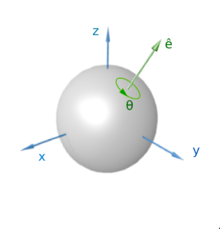
\includegraphics{Ball.png}
\end{center}
}

\frame{
https://upload.wikimedia.org/wikipedia/commons/thumb/5/51/Euler\_AxisAngle.png/220px-Euler\_AxisAngle.png
}
\end{document}
